\documentclass[a4paper]{article}

\usepackage{fullpage} % Package to use full page
\usepackage{parskip} % Package to tweak paragraph skipping
\usepackage{tikz} % Package for drawing
\usepackage{amsmath}
\usepackage{hyperref}
\usepackage{listings}

\tikzset{
  treenode/.style = {shape=rectangle, rounded corners,
                     draw, align=center,
                     top color=white, bottom color=blue!20},
  root/.style     = {treenode, font=\Large, bottom color=red!60},
  env/.style      = {treenode, font=\ttfamily\normalsize},
  dummy/.style    = {circle,draw},
  error/.style	  = {dummy,fill=red},
  sol/.style	  = {dummy,fill=green},
  useless/.style  = {dummy,fill=blue}
}

\title{Backtracking}
\author{Parallel Computing\\\\\emph{Swasti Kakker}\\\emph{Ashutosh Bhatt}\\\emph{Prabodh Agarwal}}
\date{Term Project}

\begin{document}

\maketitle

\section{Backtracking}

Backtracking is a refinement on brute-force approach. Systematically a space of possible values for given problem is searched to generate a solution(s). It is assumed that solution values are available as a vector of values. A permutation of these values is explored in a depth first manner until a possible solution is found.

Initially, the solution vector is empty. At every stage of traversal, the vector is extended with a new value generating a partial vector. If the partial vector can't be extended anymore and the problem is not yet solved, the algorithm \emph{backtracks} to replace last added values until a new value fits in the partial solution, thereby forming a branch in the tree.

Existence of a path from root to solution with decisions based on different values at tree edge and partial solutions at internal nodes, a \emph{backtracking} solution, thus forms a tree.

\begin{lstlisting}
ALGORITHM try(v1,...,vi)
	IF (v1,...,vi) is a solution THEN RETURN (v1,...,vi) 
   	FOR each v DO 
   		IF (v1,...,vi,v) is acceptable vector  THEN 
        	sol = try(v1,...,vi,v) 
        IF sol != () THEN RETURN sol 
        END 
   END 
   RETURN ()
\end{lstlisting}
\begin{figure}[!htbp]
\begin{center}
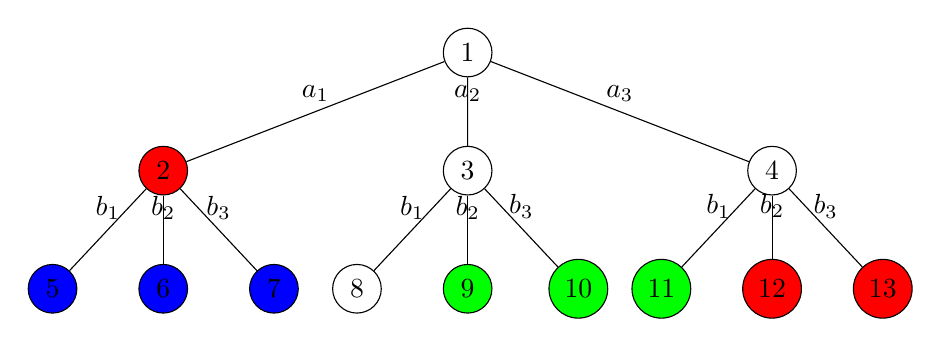
\begin{tikzpicture}
\tikzstyle{level 1}=[sibling distance=11em]
\tikzstyle{level 2}=[sibling distance=4em]
\tikzstyle{level 3}=[sibling distance=2em]
  [
    grow                    = down,
    level distance          = 6em,
    edge from parent/.style = {draw, -latex},
    every node/.style       = {font=\footnotesize},
    sloped
  ]

	\node [dummy] {1}
    child { node [error] {2}
		child { node [useless] {5} edge from parent node [above] {$b_{1}$} }
        child { node [useless] {6} edge from parent node [above] {$b_{2}$} }
        child { node [useless] {7} edge from parent node [above] {$b_{3}$} }    
    edge from parent node [above] {$a_{1}$} }
    child { node [dummy] {3}
        child { node [dummy] {8} edge from parent node [above] {$b_{1}$} }
        child { node [sol] {9} edge from parent node [above] {$b_{2}$} }
        child { node [sol] {10} edge from parent node [above] {$b_{3}$} }
    edge from parent node [above] {$a_{2}$} }     
    child { node [dummy] {4}
        child { node [sol] {11} edge from parent node [above] {$b_{1}$} }
        child { node [error] {12} edge from parent node [above] {$b_{2}$} }
        child { node [error] {13} edge from parent node [above] {$b_{3}$} }
    edge from parent node [above] {$a_{3}$} };
  
\end{tikzpicture}
\end{center}
\caption{Depiction of a backtracking search tree. Node 2 is not a valid solution thus, nodes 5,6 and 7 are never calulated. Similarly, nodes 12 and 13 are not in solution space. Nodes 9,10 and 11 are solutions. Node 8 is still being calulated and may spawn more branches.}\label{backfig}
\end{figure}

From fig.\ref{backfig}, we can see there are \emph{three} possible solutions to the problem in consideration. They are $\{a_{2}, b_{2}\}$, $\{a_{2},b_{3}\}$ and $\{a_{3},b_{1}\}$. Thus, each path from root to \emph{green} node is one solution. Also, input $a_{1}$ goes to node 2 however, it turns out that this solution is invalid thus nodes 5,6,7 are never formed.

This causes \emph{backtrack} and solution search replaces $a_{1}$ with $a_{2}$ and proceeds to node 3 and so on. Close analysis of this search tree clearly shows how path formation is independent of one another and that a solution space starting $a_{1}$ is independent of that starting at $a_{2}$. There is inherent parallelism in this problem solving approach which can be extracted by spawning paths leading to sibling nodes at once in parallel.

For example,\\
Edges $(1,2)$, $(1,3)$ and $(1,4)$ can be spawned in parallel. Nodes 2,3 and 4 can further spawn their children edges in this manner and so on.

\section{Problems}
For our term project, we have selected two problems to demonstrate backtracking.
\begin{itemize}
\item{Nqueens generator}
\item{CNF-SAT solver}
\end{itemize}
Following sections outline in detail for each problem
\begin{itemize}
\item{Explanation of problem statement}
\item{Extracting parallel structure of problem through backtracking}
\item{Explain a backtracking algorithm}
\item{Designing parallel solution using \emph{Foster's Design Methodology}}
\end{itemize}

\section{N-Queens Generator}
\subsection*{Problem Statement}
Given a NxN chessboard, find a way to place \emph{N queens} on the board in such a way that no queen cross the other. Thus, a solution requires that no two queens share the same row, column, or diagonal. We are aiming to generate all possible solutions for the N Queens Problem.
\begin{figure}[ht!]
\centering
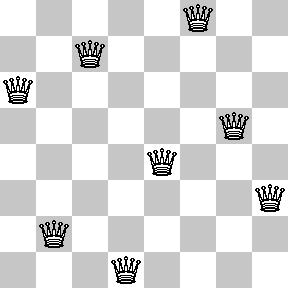
\includegraphics[width=50mm]{a.png}
\caption{An 8x8 NQueens.\label{overflow}}
\label{fig:nqueens}
\end{figure}
\subsection*{Algorithm}
The solution space for the N queens problem would clearly be $\{1, 2, 3,\dots,N\}$. Thus, trying all vectors $(p_{1},p_{2},\dots, p_{n})$ implies $n^n$ cases. Noticing that all the queens must reside in different row reduces the number of cases to $n!$.  Thus we will try to keep a queen in each of the rows.

Let us take up the 4x4 Queens problem for understanding the algorithm. Fig \ref{fig:partialq} is a partial graph indicating the tasks required.
\begin{figure}[ht!]
\centering
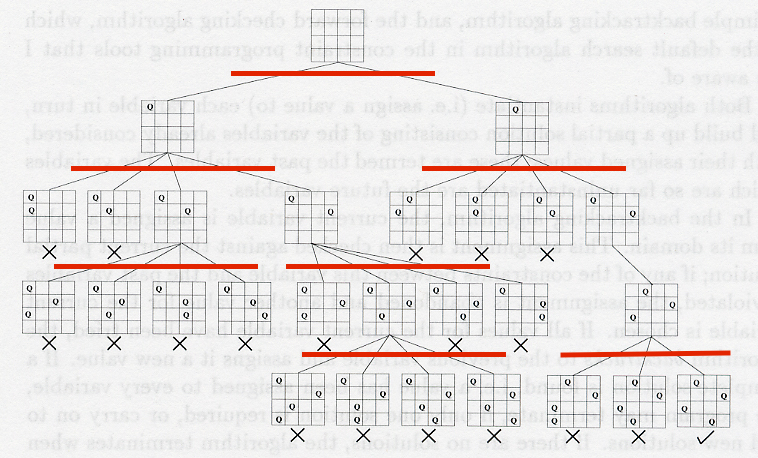
\includegraphics[width=130mm]{b.jpg}
\caption{An partial NQueens solution.\label{overflow}}
\label{fig:partialq}
\end{figure}
Thus, at the root node of our tree, we will make the decision of placement of the first queen in the first row. The nodes indicate position where the queen is placed. Each level, indicates the row in which the queen is to be placed in that level.

Clearly, when we place a new queen we check if we can continue placing new queens or should we halt. Checking this would involve if we would be able to place N queens subsequently on the board due to placement of that queen. If this is not the case, we shall abandon going down the tree further. Such nodes are marked by crosses in the partial graph.

\begin{lstlisting}
FOR R=1 to N
	TRY placement of queen for row R in each of the N positions
	(column 1 to N )concurrently.
	IF this placement could lead to a valid board configuration,
	then increment R and repeat.
    ELSE break.
\end{lstlisting}
\subsection*{Foster's Design}
\subsubsection*{Partitioning}
The number of valid positions we can place a queen, will be different tasks. Now for that valid entry, we'll have multiple branches (and hence different sibling tasks) depending on the number of valid positions left for us to place queens.  This is how the partitioning is being done. Each of the tasks can execute in parallel. The sibling tasks are independent of each other.
\subsubsection*{Communication}
As earlier stated, the sibling tasks are independent of each other, hence not much communication is required between the sibling tasks. The only communication required is between: parent task and child tasks,i.e. every parent task communicates state of the board to children tasks.
\subsubsection*{Agglomeration}
We can here intuitively realize that a parent task when communicating the board information to its children (say n), is sending the same message n times. To reduce redundancy, we implement a shared memory model. The parent task may send the current board position to all the children tasks. Hence, the number of messages passed will be low but frequent.
\subsubsection*{Mapping}
Given, p processors, and t threads per processor, first p tasks will be sent to individual processors. Subsequent tasks will be kept on a task pool of individual process. The processor picks tasks from this task pool. Now there is high probability that that a particular processor is idle while other processors are busy. Each processor has a decentralized manager, which requests tasks from the task pool of idle processors if the processor is idle.
\section{CNF-SAT Solver}
\subsection*{Problem Statement}
The \emph{Satisfiability Problem (SAT)} is a combinatorial problem. Given a Boolean formula of \emph{n} variables $$f(x_{1},x_{2},\dots,x_{n}),$$ values need to be supplied in a manner, the formula evaluates to true.

The \emph{CNF Satisfiability Problem (CNF-SAT)} is a version of the Satisfiability Problem where, the boolean formula is specified as a Conjunction of \emph{clauses}, and each clause is a disjunction of \emph{literals}. A literal is a variable or its negation. It is an AND of ORs. Example: $$(x_{1} \lor x_{2})\land(\neg x_{2} \lor x_{3} \lor \neg x_{4})\land(\neg x_{1} \lor x_{4})$$
An assignment of $x_{1} = true, x_{2} = false, x_{3} = false, x_{4} = true$ \emph{satisfies} the above formula. There can be a few more distinct assignments of $x_{i}s$ to satisfy this formula.

We are aiming generating all possible solutions to any given formula.
\subsection*{Algorithm}
Each of $x_{1-4}$ can take possible values of \emph{true} or \emph{false} thereby giving $2^{4}$ possible solutions to test on and a search space of \emph{16} values.

The backtracking solution to CNF-SAT is given by the \emph{Davis-Putnam-Logemann-Loveland}(DPLL) algorithm\cite{dpll}. The backtracking algorithm builds a tree by choosing a \emph{true} or a \emph{false} value for a literal and then simplifying the clause in a manner as given in DPLL.
\begin{lstlisting}
Repeat
	Select a literal l (some x or x')
	F = Simplify(F, l)
	While F contains a 1-clause l'
		F = Simplify(F, l')
	If all clauses removed return SAT
	If there is a 0-clause
		Backtrack to last free step and flip assignment
\end{lstlisting}

Simplify(F, l) works as
\begin{itemize}
\item{} remove clauses containing l
\item{} from all other clause, remove l' 
\end{itemize}

Application of Simplify(F, l) to unit-clause is called \emph{Unit-propagation}.

Following figure \ref{fig:cnfsat} shows formation of backtracking tree for given formula by above mentioned algorithm.
$$(\neg x_{1} \lor \neg x_{2})\land(x_{1} \lor \neg x_{2})\land(\neg x_{1} \lor \neg x_{3})$$

\begin{figure}[!htbp]
\begin{center}
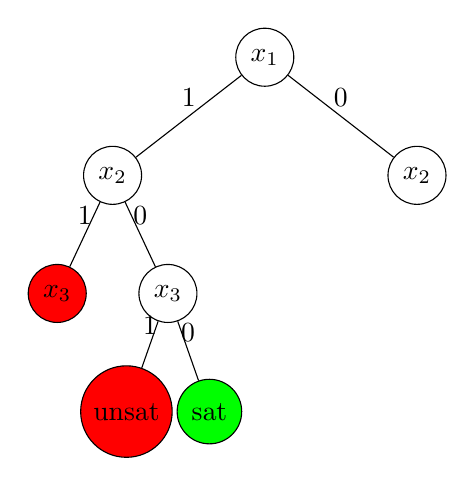
\begin{tikzpicture}
\tikzstyle{level 1}=[sibling distance=11em]
\tikzstyle{level 2}=[sibling distance=4em]
\tikzstyle{level 3}=[sibling distance=3em]
  [
    grow                    = down,
    level distance          = 6em,
    edge from parent/.style = {draw, -latex},
    every node/.style       = {font=\footnotesize},
    sloped
  ]

	\node [dummy] {$x_{1}$}
    child { node [dummy] {$x_2$}
		child { node [error] {$x_{3}$} edge from parent node [above] {1} }
        child { node [dummy] {$x_{3}$} 
        	child { node [error] {unsat} edge from parent node [above] {1}}
        	child { node [sol] {sat} edge from parent node [above] {0}}        
        edge from parent node [above] {0} }    
    edge from parent node [above] {1} }
    child { node [dummy] {$x_{2}$} edge from parent node [above] {0} };
  
\end{tikzpicture}
\end{center}
\caption{Depiction of a backtracking search tree for CNF-SAT. More solutions can be possible if $x_{1} = false$ is explored in a similar manner.}\label{fig:cnfsat}
\end{figure}

Thus each edge of the tree corresponds to assignment to a particular literal and accordingly, simplification of the formula. Each node is output of the decision indicating if the partial solution can satisfy the formula or not.

A parallel implementation of this algorithm will spawn both tasks of literals being \emph{true} and \emph{false} together. If at a level \emph{i}, a partial solution of assignments $x_{1}$ to $x_{i}$ causes one or more clauses to become 0, that path is stopped from spawning more tasks. The fact that each path of the tree is independent of sibling paths permits us to construct edges in parallel so as to perform an exhaustive search of the solution space.
\subsection*{Foster's Design}
\subsubsection*{Partitioning}
The parallel algorithm selects one literal per task depending on the tree level. Tasks are uniform with each getting a literal depending on state of it parent task and simplifying the clause based on that task. The nature of problem is fine-grained and no partitioning shall be required \cite{foster}.
\subsection*{Communication}
The edges of the tree are the tasks and also depict a communication direction as each task communicates the formula to spawned tasks and info on literals still left to be assigned. Communication is uniform and a 2-time affair.
\begin{itemize}
\item{} First when newly formed task receives from parent task
\item{} When a task communicates the formula to children tasks.
\end{itemize}
\subsubsection*{Agglomeration}
Due to each task communicating its state to children tasks, and tasks themselves being fairly easy to compute, instances of communication would be high. Same data shall be communicated by a task to two children tasks. This shows involvement of three tasks on same data, thus, all three of these tasks should implement shared memory to reduce message passing communication, and thereby keep time spent in message passing in check.
\subsubsection*{Mapping}
Given, \emph{p} processors, and \emph{t} threads per processor, first p tasks shall be sent to individual processors. Subsequent tasks on a given processor shall be kept on a task pool. The processor shall pick tasks from this task pool. As depicted in \ref{fig:cnfsat}, leftmost task finishes earlier and there is high probability that that particular processor is idle while other processors are busy. Each processor has a decentralized manager, which requests tasks from the task pool of idle processors \cite{foster}.
\bibliographystyle{plain}
\bibliography{bibliography}
\end{document}